\documentclass[12pt]{article}
\usepackage[margin=0.7in]{geometry}
\usepackage{graphicx}
\usepackage{amsmath}
\usepackage{float}
\usepackage{capt-of}
\usepackage{varwidth}
\usepackage{booktabs}
\usepackage{comment}

% Define a command to layout a table
% Inpute values are #1 input layer bias node
%                   #2 hidden layer bias node
%                   #3 standardization of features
%                   #4 PCA applied
%                   #5 Testing Accuracy
%                   #6 Table Caption
\newcommand{\testingAccuracyTable}[6] {
  \begin{tabular}{l|l}
    \hline
    Input layer bias node & #1 \\
    Hidden layer bias node & #2 \\
    Standardization of features & #3 \\
    PCA applied & #4 \\
    \hline
    Testing Accuracy & #5 \\
    \hline
  \end{tabular}
  ~\\[60pt]
  \caption{#6}
}

% Define a command to layout a table and plot
% Inpute values are #1 input layer bias node
%                   #2 hidden layer bias node
%                   #3 standardization of features
%                   #4 PCA applied
%                   #5 Testing Accuracy
\newcommand{\testingAccuracyTableAndPlot}[5] {
  \begin{center}
    \begin{table}[H]
      \begin{varwidth}[b]{0.4\linewidth}
        \centering
        \testingAccuracyTable{#1}{#2}{#3}{#4}{#5}{#1#2#3#4 Testing Accuracy}
        \label{table:#1#2#3#4}
      \end{varwidth}%
      \hfill
      \begin{minipage}[b]{0.6\linewidth}
        \centering
        \includegraphics[width=100mm]{./accuracy_imgs/#1#2#3#4_training_accuracy.png}
        \captionof{figure}{#1#2#3#4 Training Accuracy}
        \label{fig:#1#2#3#4}
      \end{minipage}
    \end{table}
  \end{center}
}

% Define a command to layout a table
% Inpute values are #1 input layer bias node
%                   #2 hidden layer bias node
%                   #3 standardization of features
%                   #4 PCA applied
%                   #5 Mean Testing Accuracy
%                   #6 Mean Validation Accuracy
%                   #7 Table Caption
\newcommand{\testingValidationAccuracyTable}[7] {
  \begin{tabular}{l|l}
    \hline
    Input layer bias node & #1 \\
    Hidden layer bias node & #2 \\
    Standardization of features & #3 \\
    PCA applied & #4 \\
    \hline
    Avg. Testing Accuracy & #5 \\
    Avg. Validation Accuracy & #6 \\
    \hline
  \end{tabular}
  ~\\[60pt]
  \caption{#7}
}

% Define a command to layout a table and plot
% Inpute values are #1 input layer bias node
%                   #2 hidden layer bias node
%                   #3 standardization of features
%                   #4 PCA applied
%                   #5 Mean Testing Accuracy
%                   #6 Mean Validation Accuracy
\newcommand{\testingValidationAccuracyTableAndPlot}[6] {
  \begin{center}
    \begin{table}[H]
      \begin{varwidth}[b]{0.4\linewidth}
        \centering
        \testingValidationAccuracyTable{#1}{#2}{#3}{#4}{#5}{#6}{#1#2#3#4 Testing Accuracy}
        \label{table:#1#2#3#4}
      \end{varwidth}%
      \hfill
      \begin{minipage}[b]{0.6\linewidth}
        \centering
        \includegraphics[width=100mm]{./accuracy_imgs/#1#2#3#4_training_accuracy.png}
        \captionof{figure}{#1#2#3#4 Training Accuracy}
        \label{fig:#1#2#3#4}
      \end{minipage}
    \end{table}
  \end{center}
}

\begin{document}

\begin{titlepage}

\newcommand{\HRule}{\rule{\linewidth}{0.5mm}} % Defines a new command for the horizontal lines, change thickness here

\center % Center everything on the page

%----------------------------------------------------------------------------------------
%	HEADING SECTIONS
%----------------------------------------------------------------------------------------

\textsc{\LARGE Drexel University}\\[1.5cm] % Name of your university/college
\textsc{\Large CS499I}\\[0.5cm] % Major heading such as course name
\textsc{\large Advanced Neural Networks}\\[0.5cm] % Minor heading such as course title

%----------------------------------------------------------------------------------------
%	TITLE SECTION
%----------------------------------------------------------------------------------------

\HRule \\[0.4cm]
{ \huge \bfseries Facial Recognition With Artificial Neural Networks}\\[0.4cm] % Title of your document
\HRule \\[1.5cm]

%----------------------------------------------------------------------------------------
%	AUTHOR SECTION
%----------------------------------------------------------------------------------------

\begin{minipage}{0.4\textwidth}
\begin{flushleft} \large
\emph{Author:}\\
Alexander \textsc{Marion}\\
Matthew \textsc{D'Amore}
\end{flushleft}
\end{minipage}
~
\begin{minipage}{0.4\textwidth}
\begin{flushright} \large
\emph{Supervisor:} \\
Dr. Matthew \textsc{Burlick}
\end{flushright}
\end{minipage}\\[4cm]

% If you don't want a supervisor, uncomment the two lines below and remove the section above
%\Large \emph{Author:}\\
%John \textsc{Smith}\\[3cm] % Your name

%----------------------------------------------------------------------------------------
%	DATE SECTION
%----------------------------------------------------------------------------------------

{\large \today}\\[3cm] % Date, change the \today to a set date if you want to be precise

%----------------------------------------------------------------------------------------
%	LOGO SECTION
%----------------------------------------------------------------------------------------

%\includegraphics{Logo}\\[1cm] % Include a department/university logo - this will require the graphicx package

%----------------------------------------------------------------------------------------

\vfill % Fill the rest of the page with whitespace
\end{titlepage}

\newpage

\section{Abstract}
Using a shallow artificial neural network and the Yale Faces Database we trained artificial neural networks in an attempt to find the optimal parameters to minimize error. Using data manipulation techniques such as standardization and principal component analysis (PCA) we were able to increase the accuracy of a shallow neural network while decreasing runtime and number of training iterations. We were able to provide reasonable bounds for the number of training iterations, hidden layer size, and image size using empirical data.


\section{Introduction}
This paper explores artificial neural networks for identifying black and white images of frontal faces with different expressions. A shallow neural network comprised of three layers (input, hidden, and output) was trained varying multiple parameters to test and the optimal parameters for the highest accuracy. The Yale Face Database which contains 165 grayscale frontal face images was used as input for training, testing, and validation.


\section{Dataset}
\textbf{Yale Faces Database} \quad This dataset contains 165 frontal grayscale images in GIF format of 15 individuals with 11 images per person. There is one image per each of the following configurations: center-light, with glasses, happy, left-light, without glasses, normal, right-light, sad, sleepy, surprised, and winking.


\section{Training Methods}
The artificial neural network was trained using forward-backward propagation which is comprised of two main steps: prediction and error propagation. Forward-backward propagation uses logistic regression to perform gradient descent to minimize the error in the output layer. The weights for each node are updated proportionally to the error at that node.\\

During forward propagation (or prediction) the input layer (in this case, image features) is used to calculate the values of the hidden layer by multiplying the input values by a matrix of weights which are initialized randomly to values between -1 and 1. As in logistic regression, these values are input to the sigmoid function which outputs a value between 0 and 1. The hidden layer is then multiplied by another matrix of weights to produce the output layer (the prediction) which are also input to the sigmoid function. The sigmoid function returns the output layer which is a collection of probabilities between 0 and 1, the highest of which is chosen as the predicted class.\\

The forward propagation process is as follows:\\
For every hidden node $j$ compute the output value using activation function $g$, the input value $x$, and the weights from the input layer to the hidden layer denoted $\beta$. For our purposes let the activation function $g$ denote the sigmoid function $g(x) = \frac{1}{1 + e^{-x}}$. The following formula gives the value at hidden node $j$:\\
$$h_j = g(x\beta_{:,j})$$
This process is repeated for each output layer node $k$. The value of the output node is computed using the output of the hidden layer $h$, the output node's vector of weights connecting to the hidden layer $\theta_{:,k}$, and the activation function $g$. The following is the formula for computing the value at output node $o$:\\
$$o_k = g(h\theta_{:,k})$$
In matrix form the forward propagation rules can simply be written as:\\
$$h = g(x\beta)$$
$$o = g(h\theta)$$
After the prediction stage has concluded the backward propagation step begins. The difference between a predicted value and the actual value is calculated as the loss at that output node. The weights between the hidden nodes and the output node are updated based on the error at that output node. The loss at each hidden node is then calculated based on the error of all output nodes scaled by the weights of the connection to the hidden node. The weights between the input layer and the hidden layer are then updated proportionally to the error traveling on the connected edges.\\
The backward propagation process is as follows:\\
The error at the each output node is calculated as
$$\delta_k = (y_k - o_k)$$
The weights between the output nodes and the hidden layer ($\theta$) are then updated proportionally to the error at the output nodes they connect to and the data traveling along that edge. This is described by the following equation:\\
$$\frac{\partial E}{\partial \theta_{j,k}} = \delta_k h_j$$
$$\theta_{j,k} = \theta_{j,k} + \frac{\eta \partial E}{\partial \theta_{i,j}} = \theta_{j,k} + \eta \delta_k h_j$$
The loss is then computed at each hidden node based on the loss of every connection to that node scaled by the weights of those connections and the data which travels across those edges. The error formula is shown below:\\
$$\delta_j = (\sum_{k=1}^{K}(\delta_k \theta_{j,k}))h_j(1-h_j)$$
The weights between the hidden layer and input layer are then updated based on the error of their connected hidden node and the data traveling along that edge. The update rule is as follows:\\
$$\beta_{i,j} = \beta_{i,j} + \eta \frac{\partial E}{\partial \beta_{i,j}} = \beta_{i,j} + \eta \delta_j x_i$$
This process was repeated over multiple training iterations and used to perform gradient descent to minimize the training error on the output nodes. The learning rate was dynamically increased and decreased based on the performance during the current training iteration as compared to past iterations. The learning rate was incremented in small amounts when the change in accuracy rose and decreased drastically when the change in accuracy fell. \cite{adaptivelearning}\\

Before training the artificial neural network four different data manipulation techniques could be applied.\\
\begin{enumerate}
\item Adding a bias node to the input layer
\item Adding a bias node to the hidden layer
\item Standardizing the data features
\item Performing PCA to retain a percentage of the feature information
\end{enumerate}

Each of the 16 variants ($2^4$ possible combinations of these manipulations) were tested.\\

The input parameters for the artificial neural network were as follows:
\begin{enumerate}
\item Number of training iterations
\item Hidden layer size
\item Image size
\item PCA field retention
\end{enumerate}

These parameters were empirically tested as shown further below.\\


\section{Testing Methods}
Every time the artificial neural network was trained the data was split across nine folds for cross validation. Each fold had 90\% training data and 10\% testing data. The training data was then split into 20\% for a validation set and 80\% for training \cite{deeplearning}. The final split across every fold was 72\% training samples, 18\% validation samples, and 10\% testing samples. The training, validation, and testing accuracies were averaged over the nine folds. This cross validation was done to avoid bias based on the selected training set and gives a better statistical model for how this testing would generalize over any training and testing set.\\


\section{Baseline Accuracy}
To create a baseline accuracy for the shallow artificial neural network on the Yale Faces Database the network was trained with the following parameters:
\begin{center}
  \begin{tabular}{l|r}
    \hline
    Training iterations & 1000 \\
    Hidden nodes & 20 \\
    Image size & 40 \\
    PCA field retention & 0.95 \\
    \hline
  \end{tabular}
\end{center}
\bigskip

The data was standardized before training, no bias nodes were added, and PCA was not performed. The following is the testing and validation accuracy for the baseline training parameters and a plot of training accuracy vs. the current training iteration.

BASELINE PLOT AND TABLE HERE

Across nine folds the baseline training parameters trained an artificial neural network which achieved $73.3918\%$ average testing accuracy and an average validation accuracy of $70.8812\%$.

\section{Variation Testing}
The following 15 pairs of tables and figures show the remaining exhaustive set of variations for data manipulation combinations before the training of the artificial neural network. Each network was trained with the following training parameters:

\begin{center}
  \begin{tabular}{l|r}
    \hline
    Training iterations & 1000 \\
    Hidden nodes & 20 \\
    Image size & 40 \\
    PCA field retention & 0.95 \\
    \hline
  \end{tabular}
\end{center}
\bigskip

Each variation was trained and cross validated on nine folds with a training, validation, and testing set as described above.

\testingValidationAccuracyTableAndPlot{N}{N}{N}{N}{0.254061}{0.214559}
\testingValidationAccuracyTableAndPlot{Y}{N}{N}{N}{0.162443}{0.157088}
\testingValidationAccuracyTableAndPlot{N}{Y}{N}{N}{0.265757}{0.249042}
\testingValidationAccuracyTableAndPlot{N}{N}{N}{Y}{0.339181}{0.302682}
\testingValidationAccuracyTableAndPlot{Y}{Y}{N}{N}{0.192658}{0.187739}
\testingValidationAccuracyTableAndPlot{Y}{N}{Y}{N}{0.721897}{0.724138}
\testingValidationAccuracyTableAndPlot{Y}{N}{N}{Y}{0.282651}{0.302682}
\testingValidationAccuracyTableAndPlot{N}{Y}{Y}{N}{0.709552}{0.697318}
\testingValidationAccuracyTableAndPlot{N}{Y}{N}{Y}{0.405133}{0.318008}
\testingValidationAccuracyTableAndPlot{N}{N}{Y}{Y}{0.946069}{0.950192}
\testingValidationAccuracyTableAndPlot{Y}{Y}{Y}{N}{0.692658}{0.724138}
\testingValidationAccuracyTableAndPlot{Y}{Y}{N}{Y}{0.318389}{0.314176}
\testingValidationAccuracyTableAndPlot{Y}{N}{Y}{Y}{0.951917}{0.954023}
\testingValidationAccuracyTableAndPlot{N}{Y}{Y}{Y}{0.940221}{0.919540}
\testingValidationAccuracyTableAndPlot{Y}{Y}{Y}{Y}{0.940221}{0.923372}

The variant with the highest accuracy was trained by adding a bias node to the input, standardizing the data, and performing PCA with a retention rate of 95\%.\\


\section{Empirical Parameter Testing}
A shallow artificial neural network was trained varying the input parameters to empirically test the effect that each parameter had on the training, testing, and validation accuracy. The four parameters which were tested were number of training iterations, image size, PCA percent field retention, and number of hidden nodes.\\
For each test the highest performing variant of the variant testing set was used. Each artificial neural network was trained with a bias node at the input layer, standardized data, and PCA applied before training.\\
\begin{enumerate}
  \item \textbf{Number of Training Iterations}\\
  The number of training iterations was varied from 1 to 10,000 in increments of 100. The artificial neural network was trained using each number of training iterations in this set and was cross validated over nine folds. The accuracy plot show below reflects the average accuracies across the nine folds. The artificial neural network was trained with an image size of 40 by 40 and 20 hidden nodes.\\
  \begin{center}
    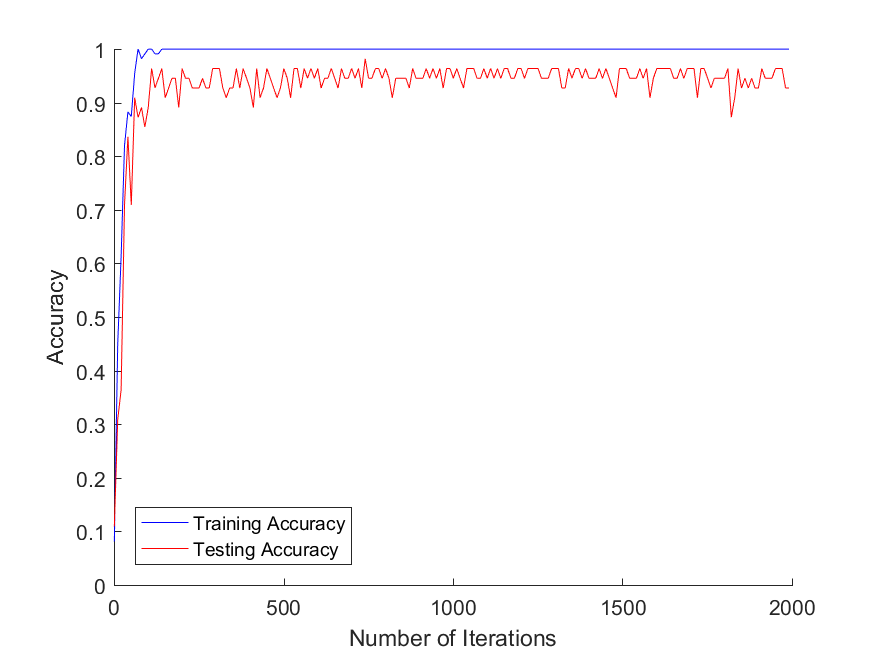
\includegraphics[width=115mm]{./figs/num_iterations_empirical.png}
    \captionof{figure}{Plot of accuracy as the number of training iterations increases}
    \label{fig:img_iters}
  \end{center}
  As shown above, the average accuracy of the artificial neural network was not dependent on the number of iterations past 300 or 400 iterations. For future testing we opted to keep our standard 1000 training iterations and adjust if we saw drastic over or underfitting.\\

  \item \textbf{Image Size and PCA Percent Field Retention}\\
  The image size and percent field retention for PCA were varied together exhaustively. Both of these variables determine the number of input nodes and are not independent of one another. The image size was varied from 10 to 100 in increments of five and the retention rate was varied from 0.10 to 1 in increments of 0.05. The artificial neural network was trained with 20 hidden nodes and 1000 training iterations.\\
  \begin{center}
    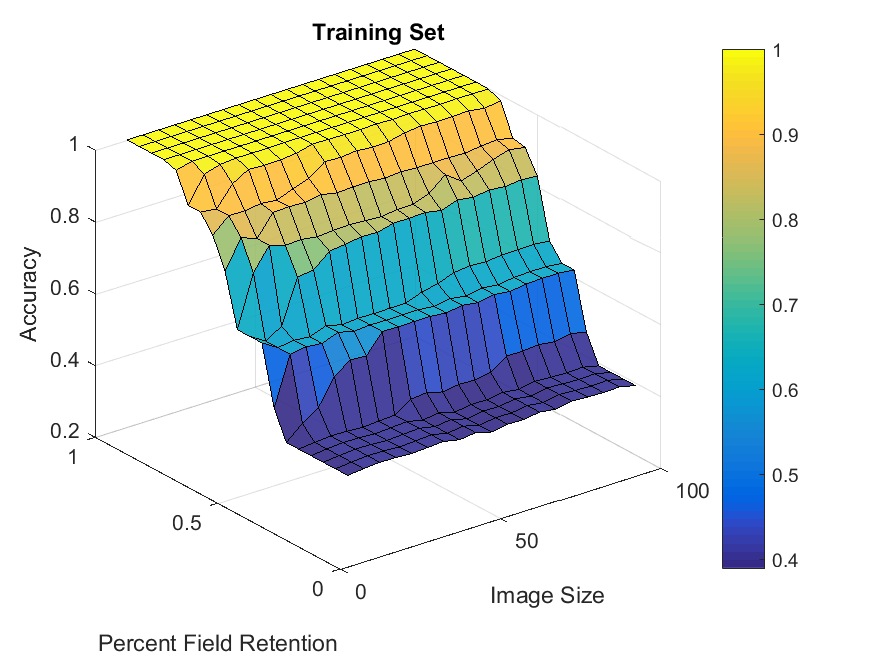
\includegraphics[width=115mm]{./figs/num_fields_empirical_training.png}
    \captionof{figure}{Plot of training accuracy as the image size and percent field retention increases}
    \label{fig:img_size_train}
  \end{center}
  \begin{center}
    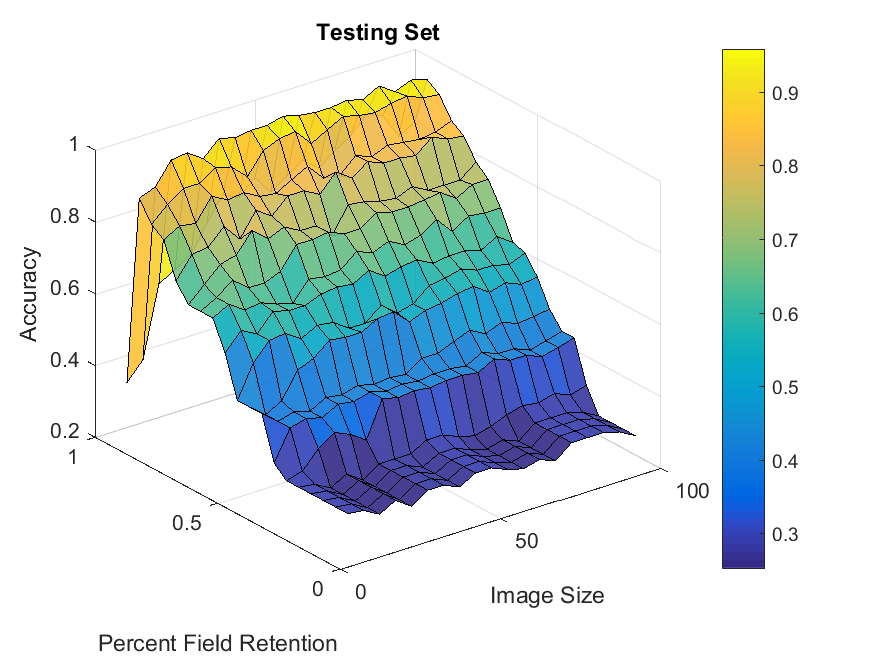
\includegraphics[width=115mm]{./figs/num_fields_empirical_testing.png}
    \captionof{figure}{Plot of testing accuracy as the image size and percent field retention increases}
    \label{fig:img_size_test}
  \end{center}
  The maximum mean testing accuracy was 95.81\% and occurred at an image size of 55 by 55 and a PCA retention rate of 0.95.\\
  \begin{center}
    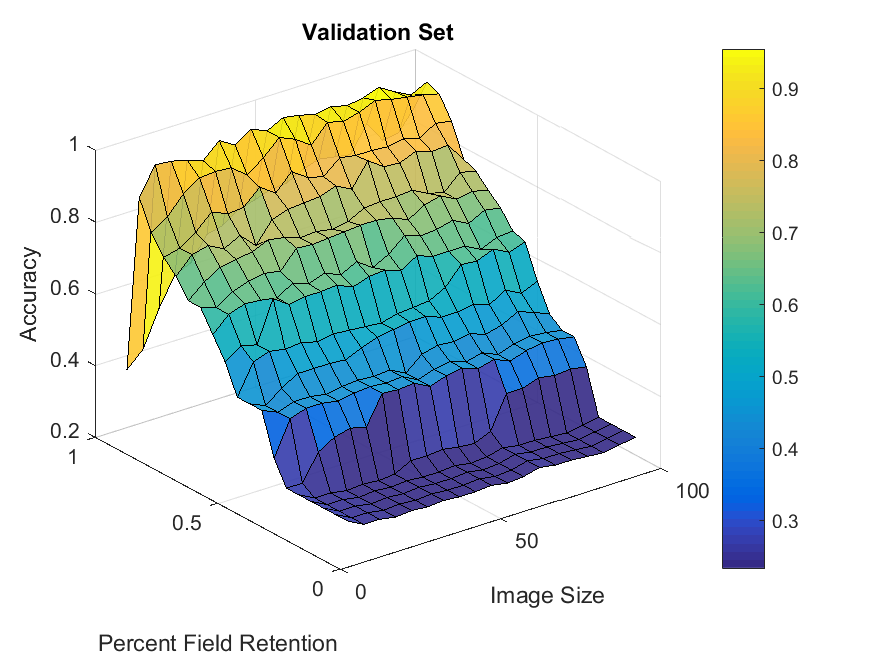
\includegraphics[width=115mm]{./figs/num_fields_empirical_validation.png}
    \captionof{figure}{Plot of validation accuracy as the image size and percent field retention increases}
    \label{fig:img_size_valid}
  \end{center}
  The maximum mean validation accuracy was 95.40\% and occurred at an image size of 55 by 55 and a PCA retention rate of 0.95.\\

  The accuracy of the artificial neural network was heavily dependent upon the image size paired with the percent field retention. The image size had less of an effect than the percent field retention which can be seen by the close to horizontal line parallel to the image size axis.\\
  \begin{center}
    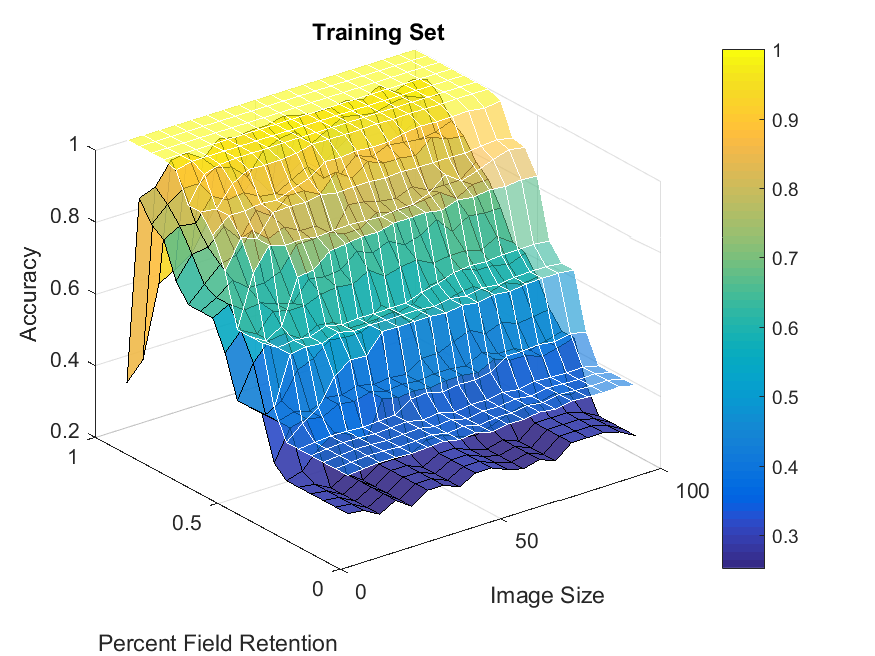
\includegraphics[width=115mm]{./figs/num_fields_empirical_training_testing_overlay.png}
    \captionof{figure}{Plot of training and testing accuracy as the image size and percent field retention increases}
    \label{fig:img_size_train_test}
  \end{center}
  \begin{center}
    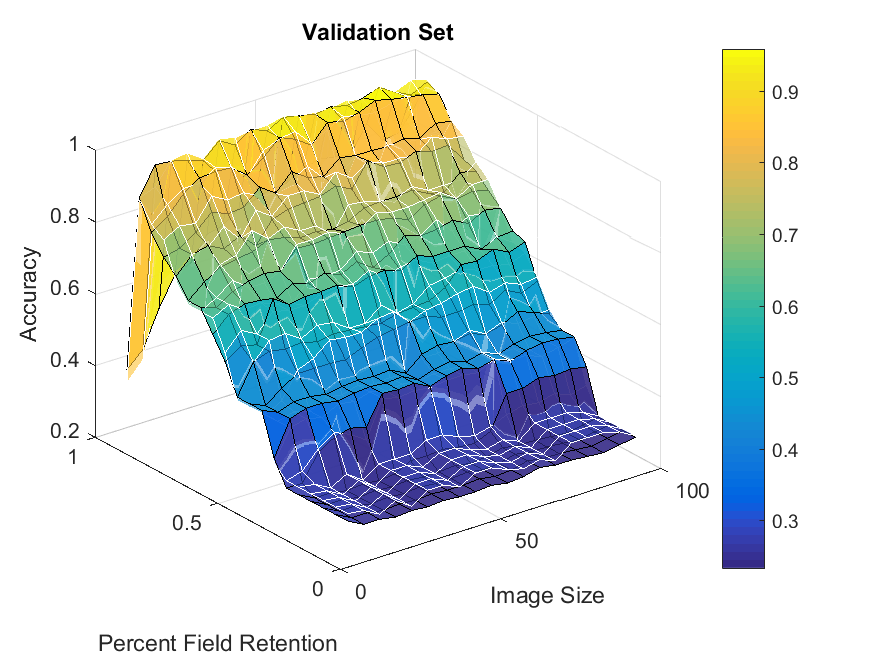
\includegraphics[width=115mm]{./figs/num_fields_empirical_validation_testing_overlay.png}
    \captionof{figure}{Plot of validation and testing accuracy as the image size and percent field retention increases}
    \label{fig:img_size_valid_test}
  \end{center}

  \item \textbf{Number of Hidden Nodes}
  The accuracy of an artificial neural network was tested with PCA applied as well as without PCA applied. The number of hidden nodes should be between the number of input nodes and the number of output nodes \cite{introNN}. The number of output nodes was 15 (one for every classifier) and the number of input nodes with PCA applied was 33 and without PCA applied was the image size squared. The artificial neural network was trained using the previously investigated optimal values for image size and percent field retention of 55 by 55 and 0.95 respectively.\\

  Without PCA the number of hidden nodes was varied from 15 to 3025 by 50. With PCA the number of hidden nodes was varied from 15 to 38 by 1.\\
  \begin{center}
    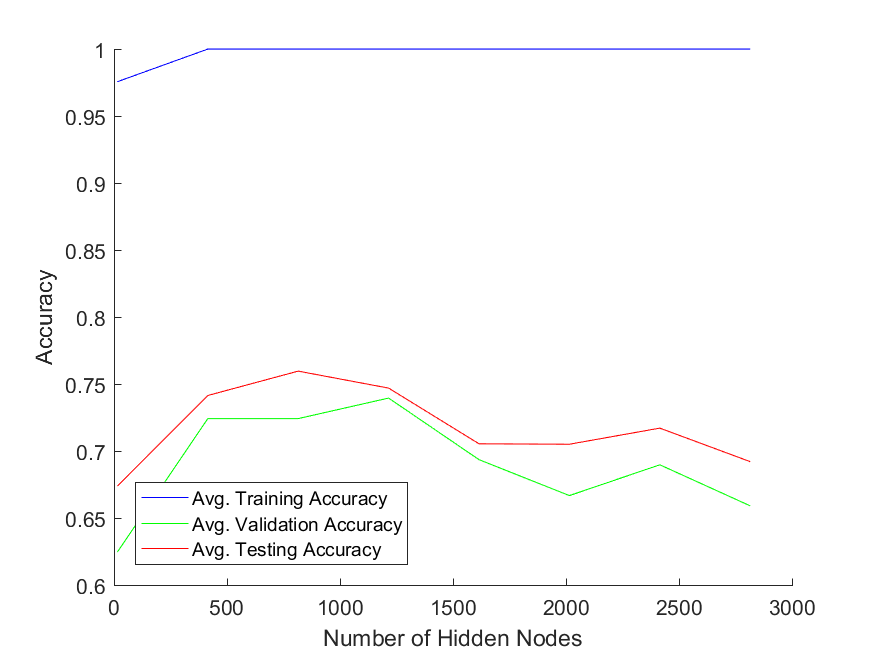
\includegraphics[width=115mm]{./figs/num_hidden_nodes_empirical.png}
    \captionof{figure}{Plot of accuracy as the number of hidden nodes increases}
    \label{fig:num_hidden_nodes}
  \end{center}
  The accuracy of the artificial neural network did not seem to be directly correlated to the number of hidden nodes in the hidden layer. With PCA applied, the mean testing accuracies varied from 0.9643 to 0.9276 and the mean validation accuracies varied between 0.9617 and 0.9119. Without PCA applied, the mean testing accuracy varied from 0.7950 and 0.6686 and the mean validation accuracy varied from 0.8102 and 0.6893.\\
\end{enumerate}

\section{Conclusions}
A shallow neural network can be used for facial recognition and classification reasonably well given some data manipulation beforehand. The most important data manipulations to increase accuracy are data standardization and PCA. Every variation that included data standardization performed markedly better than those that did not. The highest valued variation that did not standardize data (NYNY) only reached a training accuracy of 40.5133\% and a validation accuracy of 31.8008\%. The parallel variation which did standardize the data (NYYY) reached a training accuracy of 94.0221\% and a validation accuracy of 91.9540\%. Similarly the highest valued variation that did not use PCA (YNYN) only reached a testing accuracy of 72.1897\% and a validation accuracy of 72.4138\%. The similar variation which used PCA (YNYY) was the highest performing variation and reached a testing accuracy of 95.1917\% and a validation accuracy of 95.4023\%.\\
\\
After the importance of PCA and data standardization was determined the number of training iterations was empirically tested. This had very little effect on the accuracy of the artificial neural network past 300 to 400 iterations. The percent field retention and image size had the largest effect on the accuracy. Depending on the image size and percent field retention the mean testing accuracy ranged from 95.81\% to 25.31\% while the mean validation accuracy ranged from 95.40\% to 23.37\%.\\
\\
The number of hidden nodes in the hidden node layer had very little effect on the accuracy of the artificial neural network. With PCA applied the range of the mean testing accuracies was between 96.43\% to 92.76\% and the mean validation accuracies varied between 96.17\% and 91.19\%.\\
\\
By combining data manipulation techniques such as data standardization and principal component analysis a shallow neural network can be trained efficiently and to a high degree of accuracy. It is important to reduce the number of features to lessen the computational complexity and exclude features which have little to no information gain.\\

\begin{thebibliography}{9}
\bibitem{deeplearning}
Goodfellow, Ian, Yoshua Bengio, and Aaron Courville. \textit{Deep learning}. Cambridge, MA: The MIT Press, 2017. Print.

\bibitem{adaptivelearning}
Ho, K.l., Y.-Y. Hsu, and C.-C. Yang. "Short Term Load Forecasting Using a Multilayer Neural Network with an Adaptive Learning Algorithm." IEEE Transactions on Power Systems 7.1 (1992): 141-49. Web.

\bibitem{frANN}
Shivdas, Ashvini E. "Face Recognition Using Artificial Neural Network." International Journal of Research in Management, Science \& Technology (2014): n. pag. Web.

\bibitem{nnbfd}
Rowley, Henry, Shumeet Baluja, and Takeo Kanade. "Neural Network-Based Face Detection". IEEE TRANSACTIONS ON PATTERN ANALYSIS AND MACHINE INTELLIGENCE 20.1 (1998): 23-38. Print.

\bibitem{introNN}
Heaton, Jeff. \textit{Introduction to Neural Networks for Java}. 2nd ed. N.p.: Heaton Research, n.d. Print.
\end{thebibliography}

\end{document}
